\documentclass[../main.tex]{subfiles}

\begin{document}

\section{Question 1} \label{sec:q1}

Calculation of the inverse of a 2 by 2 matrix is shown below.

$$
A =
\begin{bmatrix}
    a & b \\
    c & d
\end{bmatrix}
, \hspace{20pt} A^{-1} = \frac{1}{|A|}
\begin{bmatrix}
    d & -b \\
    -d & a
\end{bmatrix}
= \frac{1}{ad - bc}
\begin{bmatrix}
    d & -b \\
    -c & a
\end{bmatrix}
=
\begin{bmatrix}
    a_\text{out} & b_\text{out} \\
    c_\text{out} & d_\text{out}
\end{bmatrix}
$$

You are to design an RTL circuit for this calculation. When \texttt{start} is asserted, \texttt{aIn}, \texttt{bIn}, \texttt{cIn}, \texttt{dIn} 16-bit busses will contain the four elements of the matrix in upper left to lower right order. When the inverse calculation is completed, the IMC (Inverse Matrix Calculator) generates a 1 on \texttt{ready} and keeps this value until a new round of calculation begins. When calculation is completed, the output data becomes available on \texttt{aOut}, \texttt{bOut}, \texttt{cOut}, \texttt{dOut} output busses. Input and output data formats are 16-bit fixed point with eight integer bits. The inputs have only integer parts, and the outputs are 16-bit data with integer and fractional parts. The input integer part should be less than or equal to 15.

You can use the following components:

\begin{itemize}
    \item 2 16-bit unisgned multipliers with 16-bit inputs and a 16-bit outputs. Each has a control signal, \texttt{select\_output}, which determines which portion of the 32-bit multiplication result is select: when $\texttt{select\_output} = 1$, the most significant 16 bits are chosen, otherwise, the bits in the range $[23:8]$ are selected. Consider the delay of this multiplier is in the order of 84d.
    \item An approximate reciprocal circuit with an unsigned 16-bit integer input and 9-bit output (1-bit integer and an 8-bit fractional). The circuit is combinational, calculates the reciprocal of its input, and has a delay of 84d.
    \item 16-bit adders, subtractors, and comparators with delay values of the order 16d.
    \item Multiplexers, decoders, and other combinational parts with delay values of the order of 1d.
    \item Registers of any size.
\end{itemize}

Design the IMC circuit such that it can operate with a clock with a period of \textbf{no more than 120d}. This limits the maximum critical path delay the circuit can have. For outputs that are negative produce a negative flag of 1.

\begin{enumerate}
    \item Create behavioural models for the multipliers and adder/subtractor.
    \item Draw the complete datapath of IMC, including the components and necessary internal control signals.
    \item Draw a state diagram showing your controller's behaviour. In each state, show the control signals that are issued.
    \item Show wiring between the datapath and the controller.
    \item Model the IMC circuit in SystemVerilog according the the schematic, datapath, and controller. \textbf{You don't need to model the delays.}
    \item Verify the design with a testbench.
\end{enumerate}

\newpage

\subsection*{Solution}

\begin{figure}[h]
    \centering
    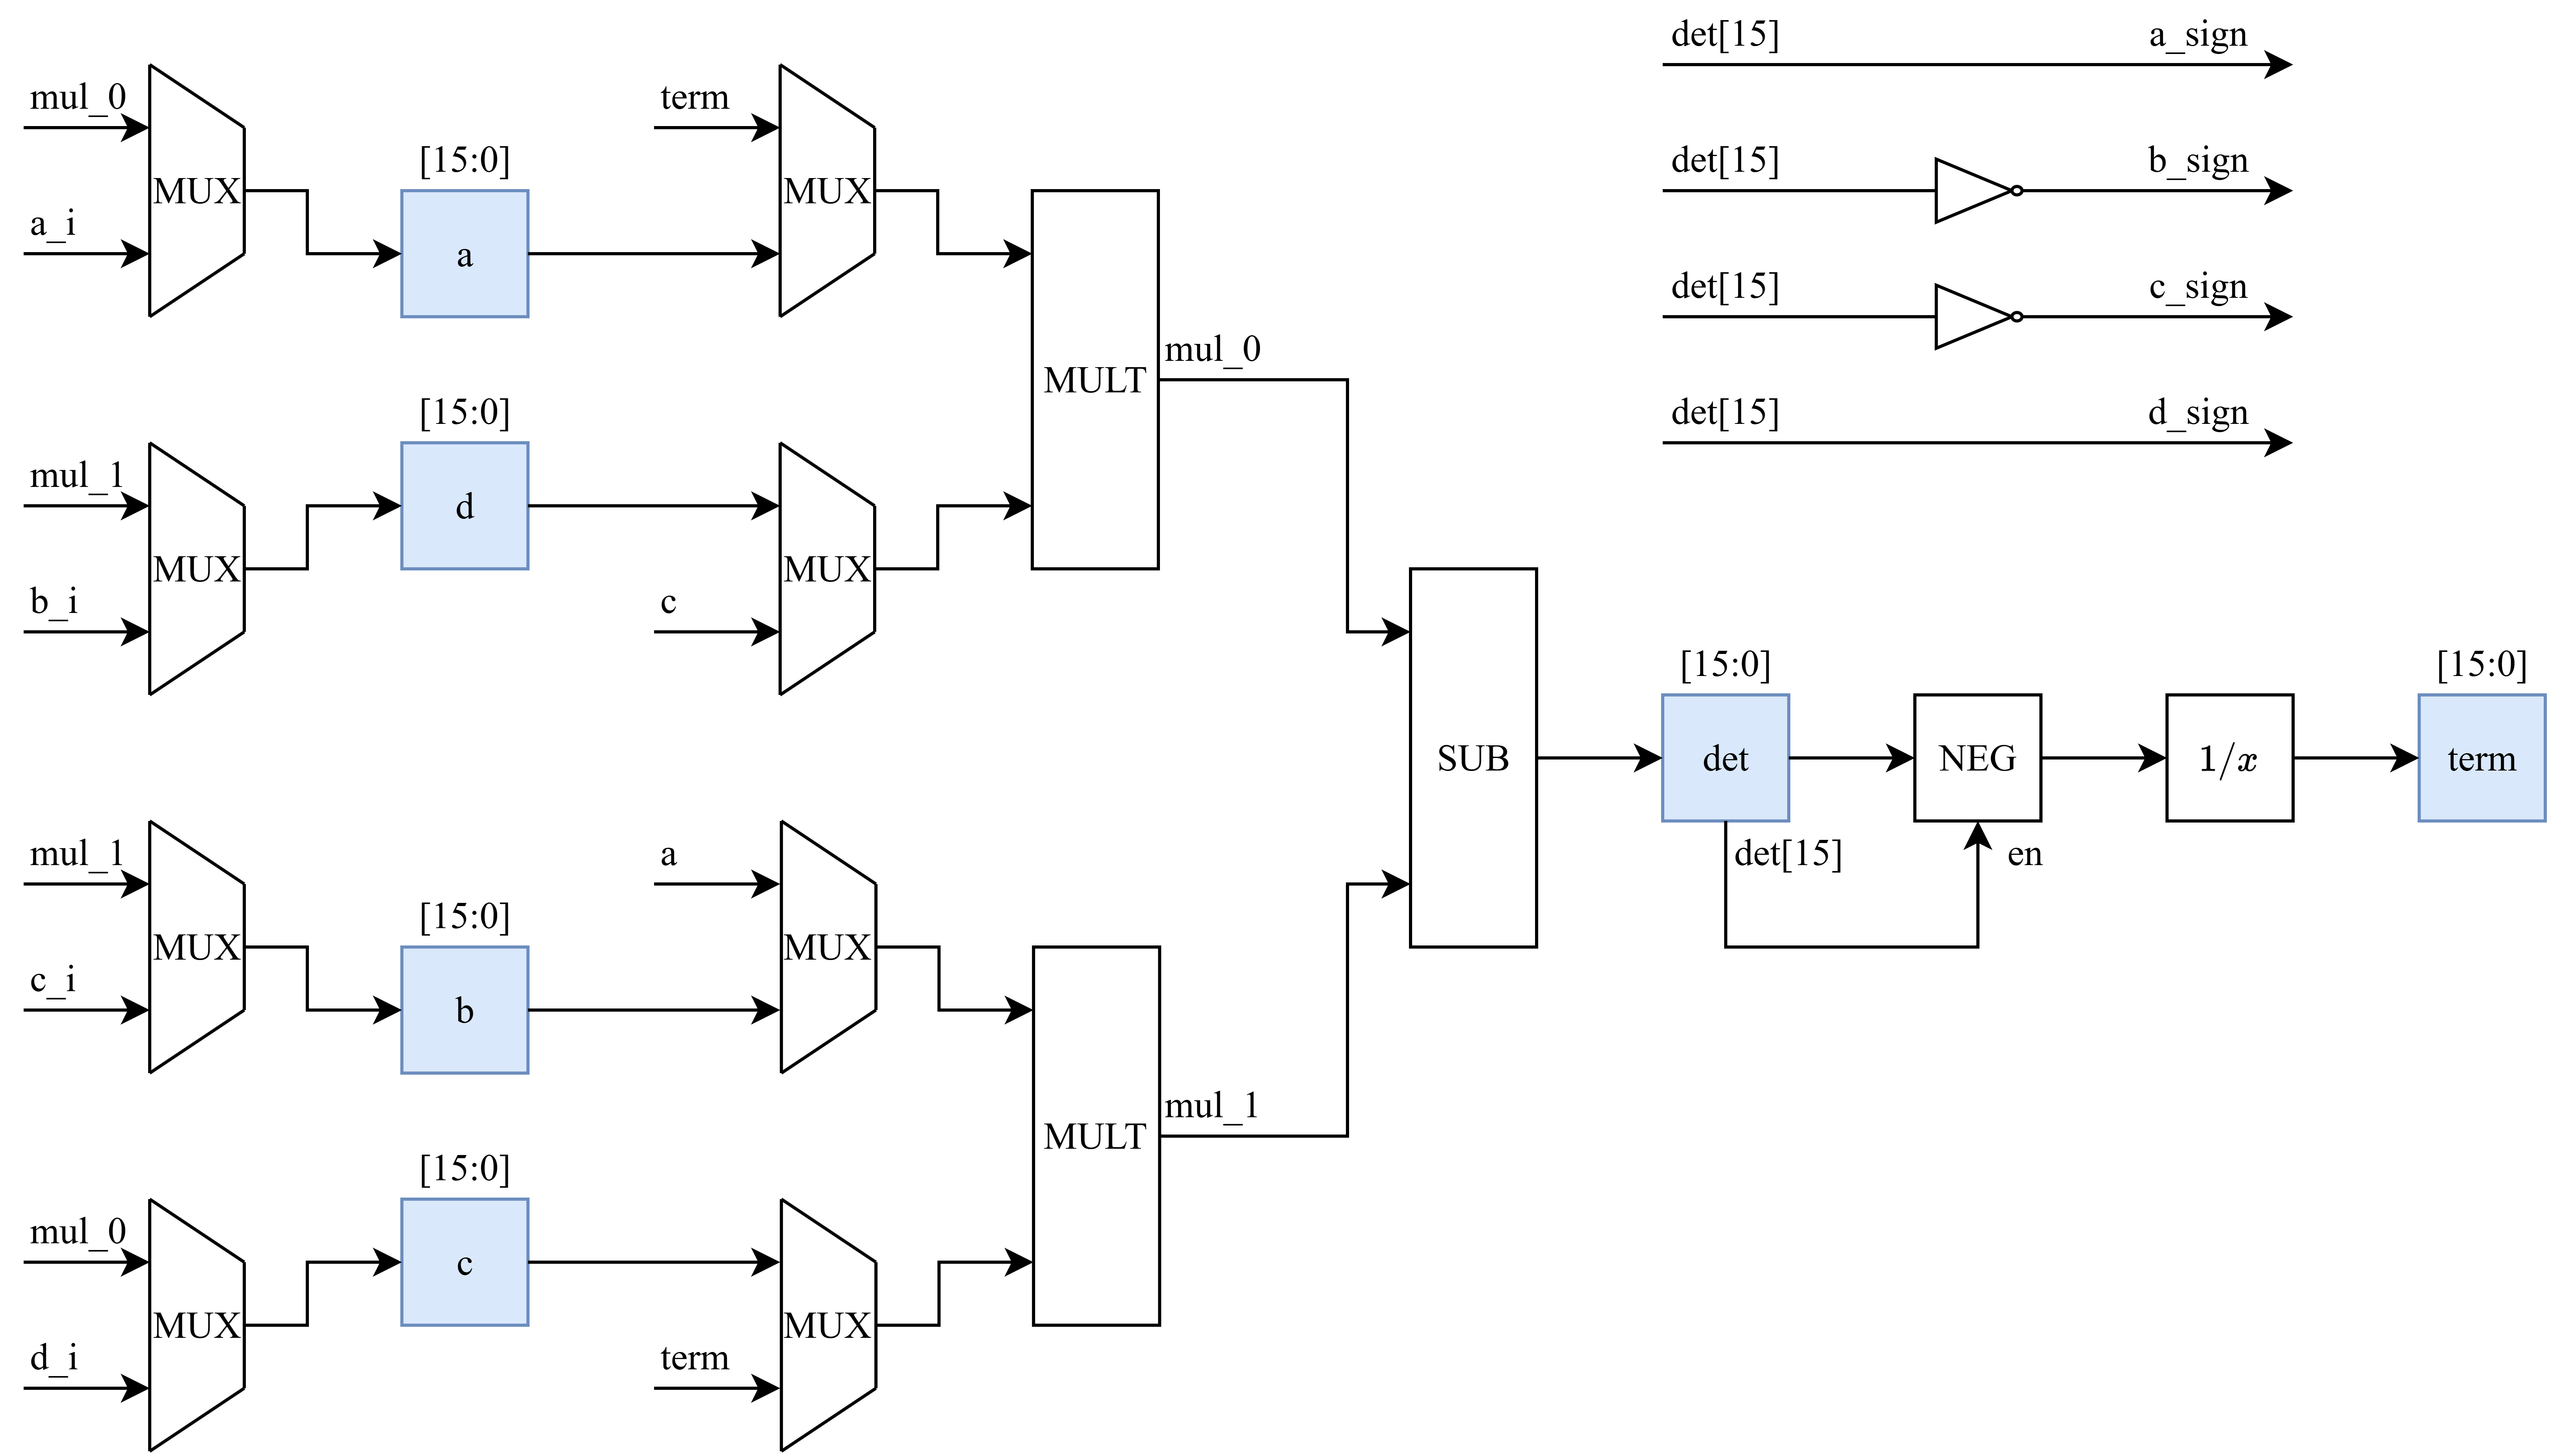
\includegraphics[width=\linewidth]{assets/q1.png}
    \caption{Datapath of IMC module. Registers are shown in blue.}
    \label{fig:q1_dp}
\end{figure}

To construct the \textit{Inverse Matrix Calculator} (IMC), we utilize 8 multiplexers, two multipliers, two adders, and one reciprocal module. To comply with the timing specifical of a maximum critical path delay of 120d, we have 6 registers (shown in blue). The datapath schematic is shown in \cref{fig:q1_dp}. The calculation consists of 5 steps corresponding directly to 5 clock cycles [\cref{tab:pipeline_cycles}].

\begin{table}[h]
    \centering
    \renewcommand{\arraystretch}{1.5}
    \setlength{\tabcolsep}{8pt}
    \begin{tabularx}{\textwidth}{@{}cX@{}}
        \toprule
        \textbf{Cycle} & \textbf{Operation} \\
        \midrule
        0 & Input values are clocked into the input/output registers \texttt{a}, \texttt{b}, \texttt{c}, and \texttt{d}. \\
        1 & The determinant, $ad - bc$, is calculated and stored in \texttt{det}. \\
        2 & If the determinant is negative, it is negated (subtractor with one operand set to 0) and the reciprocal is computed and stored in \texttt{term}. \\
        3 & Half of the inverse matrix, \texttt{aOut} and \texttt{dOut}, is computed and stored in the \texttt{a} and \texttt{d} registers. \\
        4 & The second half of the inverse matrix, \texttt{bOut} and \texttt{cOut}, is computed and stored in the \texttt{b} and \texttt{c} registers. \\
        \bottomrule
    \end{tabularx}

    \caption{Pipeline operation by clock cycle.}
    \label{tab:pipeline_cycles}
\end{table}

The sign of each entry in the inverse matrix result is computed directly from the sign of the determinant. The control signals needed for the datapath are summarized in \cref{tab:q1_control}. They consist entirely of 1-bit signals to control the registers and muxes. The longest path delay consists of the route from the input registers to the \texttt{det} register with a total delay of $1d + 84d + 16d = 101d$. The controller has a total of 7 states. Their transitions are shown in \cref{fig:q1_controller}.

\newpage

\begin{table}[h]
    \centering
    \renewcommand{\arraystretch}{1.2}
    \setlength{\tabcolsep}{8pt}

    \begin{tabularx}{\textwidth}{@{}lX@{}}
        \toprule
        \textbf{Signal} & \textbf{Description} \\
        \midrule
        \texttt{en\_a}          & Enable synchronized writing into the \texttt{a} register. \\
        \texttt{en\_b}          & Enable synchronized writing into the \texttt{b} register. \\
        \texttt{en\_c}          & Enable synchronized writing into the \texttt{c} register. \\
        \texttt{en\_d}          & Enable synchronized writing into the \texttt{d} register. \\
        \texttt{en\_det}        & Enable synchronized writing into the \texttt{det} register. \\
        \texttt{en\_term}       & Enable synchronized writing into the \texttt{term} register. \\
        \texttt{sel\_a}         & Input register mux. 1'b0: \texttt{a\_i}, \hspace{20pt} 1'b1: \texttt{mul\_0}. \\
        \texttt{sel\_b}         & Input register mux. 1'b0: \texttt{b\_i}, \hspace{20pt} 1'b1: \texttt{mul\_1}. \\
        \texttt{sel\_c}         & Input register mux. 1'b0: \texttt{c\_i}, \hspace{20pt} 1'b1: \texttt{mul\_0}. \\
        \texttt{sel\_d}         & Input register mux. 1'b0: \texttt{d\_i}, \hspace{20pt} 1'b1: \texttt{mul\_1}. \\
        \texttt{sel\_mul\_a\_0} & Multiplier 0 mux. \hspace{5pt} 1'b0: \texttt{a}, \hspace{35pt} 1'b1: \texttt{term}. \\
        \texttt{sel\_mul\_b\_0} & Multiplier 0 mux. \hspace{5pt} 1'b0: \texttt{b}, \hspace{35pt} 1'b1: \texttt{c}. \\
        \texttt{sel\_mul\_a\_1} & Multiplier 1 mux. \hspace{5pt} 1'b0: \texttt{c}, \hspace{35pt} 1'b1: \texttt{a}. \\
        \texttt{sel\_mul\_b\_1} & Multiplier 1 mux. \hspace{5pt} 1'b0: \texttt{d}, \hspace{35pt} 1'b1: \texttt{term}. \\
        \bottomrule
    \end{tabularx}

    \caption{Control signals for IMC datapath.}
    \label{tab:q1_control}
\end{table}

\vspace{-10pt}
\begin{figure}[h]
    \centering
    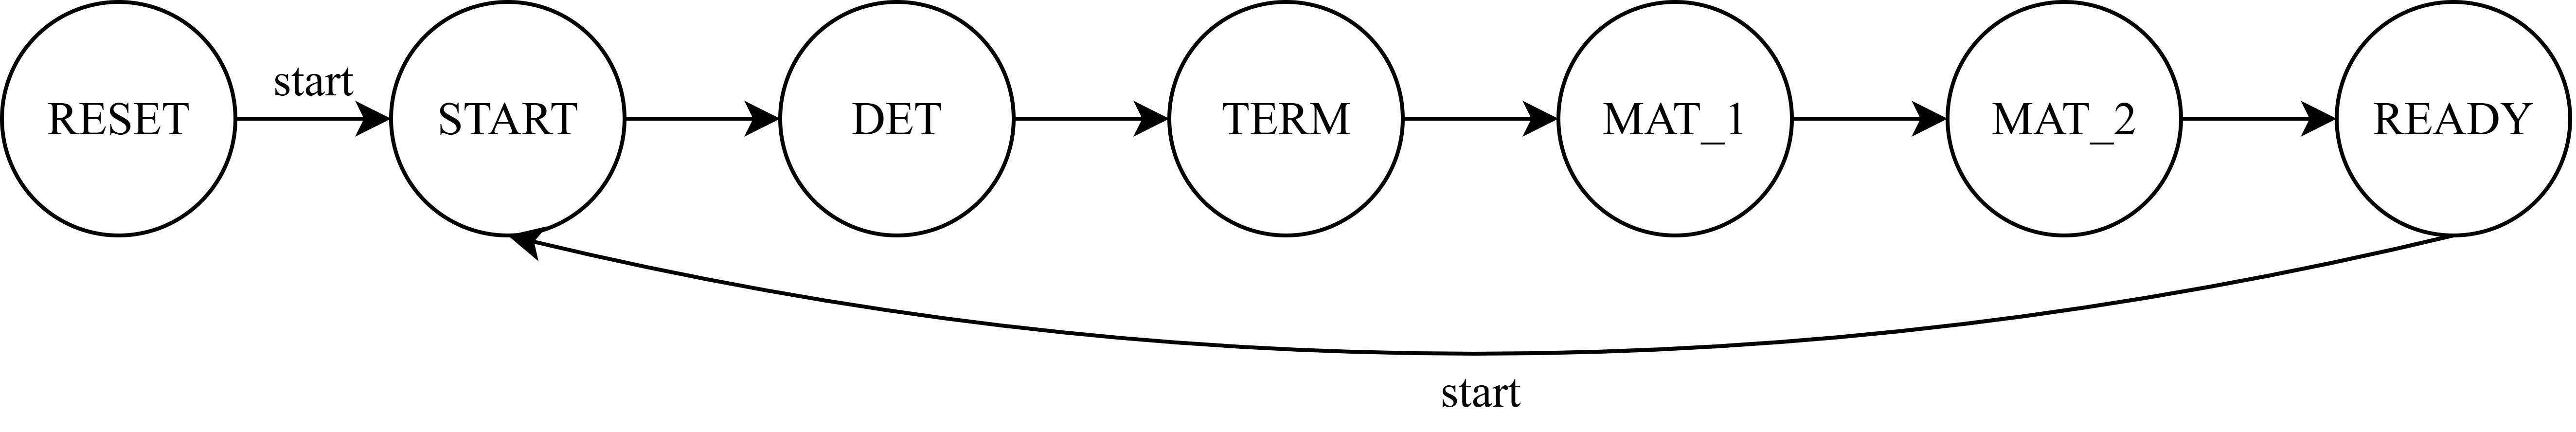
\includegraphics[width=\linewidth]{assets/q1_state.png}
    \caption{State transition diagram for IMC controller.}
    \label{fig:q1_controller}
\end{figure}

% \vspace{-10pt}
The control signals issued in each state are summarized in \cref{tab:q1_state_signals}. Finally for verification we create a testbench that input all combinations of integer values in the range $[0, 15]$ and check the result against a software implementation. It is important to note that for input values that result in a determinant above 15, the given reciprocal module doesn't work anymore and gives invalid values. Therefore such tests are skipped. A snippet of the testbench output is shown below. It passes with 0 errors with a tolerance of $0.041$ against the true software result.

\begin{textcode}{q1 - IMC testbench output}
Matrix: [[15, 9], [6, 3]]
HW inv: [-0.3281, 0.9844; 0.6562, -1.6406]
Ref inv: [-0.3333, 1.0000; 0.6667, -1.6667]

Matrix: [[15, 9], [6, 4]]
HW inv: [0.6562, -1.4766; -0.9844, 2.4609]
Ref inv: [0.6667, -1.5000; -1.0000, 2.5000]

...

[861270] Completed with 0 errors...
\end{textcode}

\newpage

\begin{table}[h]
    \centering
    \renewcommand{\arraystretch}{1.5}
    \setlength{\tabcolsep}{6pt}

    \begin{tabularx}{\textwidth}{@{}l X@{}}
        \toprule
        \textbf{State} & \textbf{Signals Active (1'b1)} \\
        \midrule
        \texttt{STATE\_START} & 
            \texttt{en\_a} \newline
            \texttt{en\_b} \newline
            \texttt{en\_c} \newline
            \texttt{en\_d} \\
        \hline
        \texttt{STATE\_DET} & 
            \texttt{en\_det} \\
        \hline
        \texttt{STATE\_TERM} & 
            \texttt{en\_term} \\
        \hline
        \texttt{STATE\_MAT\_1} & 
            \texttt{en\_a} \newline
            \texttt{en\_d} \newline
            \texttt{sel\_a} (mul\_0) \newline
            \texttt{sel\_d} (mul\_1) \newline
            \texttt{sel\_mul\_a\_0} (term) \newline
            \texttt{sel\_mul\_a\_1} (a) \newline
            \texttt{sel\_mul\_b\_1} (term) \\
        \hline
        \texttt{STATE\_MAT\_2} & 
            \texttt{en\_b} \newline
            \texttt{en\_c} \newline
            \texttt{sel\_b} (mul\_1) \newline
            \texttt{sel\_c} (mul\_0) \newline
            \texttt{sel\_mul\_a\_0} (term) \newline
            \texttt{sel\_mul\_b\_0} (c) \newline
            \texttt{sel\_mul\_b\_1} (term) \\
        \hline
        \texttt{STATE\_READY} & 
            \texttt{ready} \\
        \bottomrule
    \end{tabularx}

    \caption{Signals issued in each state.}
    \label{tab:q1_state_signals}
\end{table}

\newpage

\section{Question 2}

In this problem, you are to design an input wrapper and an output wrapper that connect the IMC circuit of the previous problem to a 16-bit arbitrated bus.

The input wrapper waits for four 16-bit data that will be handshaked to it using a two-line \texttt{dataReady}, \texttt{dataAccept} fully responsive handshaking scheme. When such is received, it checks if the IMC circuit is ready to receive its four 16-bit inputs by monitoring the IMC's \texttt{ready} output. If so, it issues a \texttt{start} signal and allows the IMC to start its operation.

The output wrapper works independently of the input wrapper. the output wrapper receives the four outputs of the IMC circuit when the IMC issues the \texttt{ready} signal. The output wrapper has an \texttt{outAvail} output that informs an external device of the availability of four 16-bit elements of the transposed matrix. When this signal is asserted, the external device may issue a start signal, \texttt{startTransmit}, to tell the output wrapper to start sending the results. The output wrapper uses \texttt{request} to get permission to use the bus, that will be responded by \texttt{grant} when the output wrapper is allowed to drive the bus. The output wrapper uses fully responsive two-line handshaking using an \texttt{outReady} output and an \texttt{outAccepted} input. The four 16-bit data outputs will be sent over the bus ina  burst fashion.

\begin{enumerate}
    \item Draw block diagrams of the input wrapper, output wrapper, and the interfacing bus, and how they wrap around the IMC circuit.
    \item Draw the datapath of the interfacing circuits, identifying control signals that are issued by the controller.
    \item Draw the state machines for the implementation of the inerface circuits controller.
    \item Model your input wrapper and output wrapper in SystemVerilog.
    \item verify your design with a testbench.
\end{enumerate}

\subsection*{Solution}

The interfacing circuits (wrappers) will convert the highly parallel data stream of the IMC module typical of intra-RTL communication, to a serialized data stream suitable for a shared bus. A schematic showing the connections to the IMC is seen in \cref{fig:q2_wrap}.

\begin{figure}[h]
    \centering
    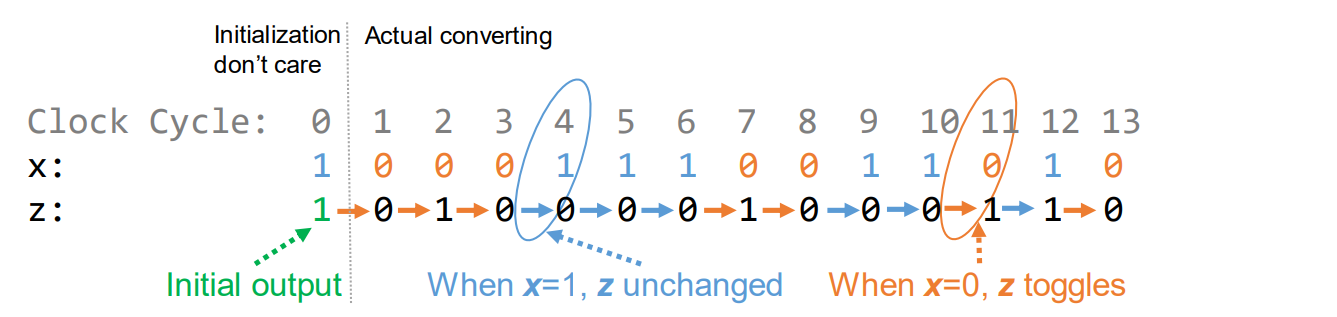
\includegraphics[width=\linewidth]{assets/q2.png}
    \caption{IMC with input and output wrappers for bus communication.}
    \label{fig:q2_wrap}
\end{figure}

\newpage

\subsection*{Input Wrapper}

The input wrapper must be able to serially read and store the four input values for the IMC. The datapath consists of only four registers to store the inputs and is shown in \cref{fig:q2_in_wrap_dp}. The datapath has four control signals [\cref{tab:q2_in_wrap_sig}]. The controller has five states: \texttt{IDLE}, \texttt{COLLECT}, \texttt{ACCEPT}, \texttt{WAIT\_IMC}, and \texttt{START\_IMC}. When the bus asserts \texttt{dataReady} the input wrapper enters the \texttt{COLLECT} state, writing the serial data into the corresponding registers. An internal counter, \texttt{data\_count}, keeps track of which register to write to. When all data has been received, the wrapper either enters a \texttt{WAIT\_IMC} if the IMC is not yet ready to receive new data. If the IMC already assets \texttt{ready}, the input wrapper directly enters the \texttt{START\_IMC} state. The state transition diagram is shown in \cref{fig:q2_in_wrap_cont}.

\begin{figure}[h]
    \centering
    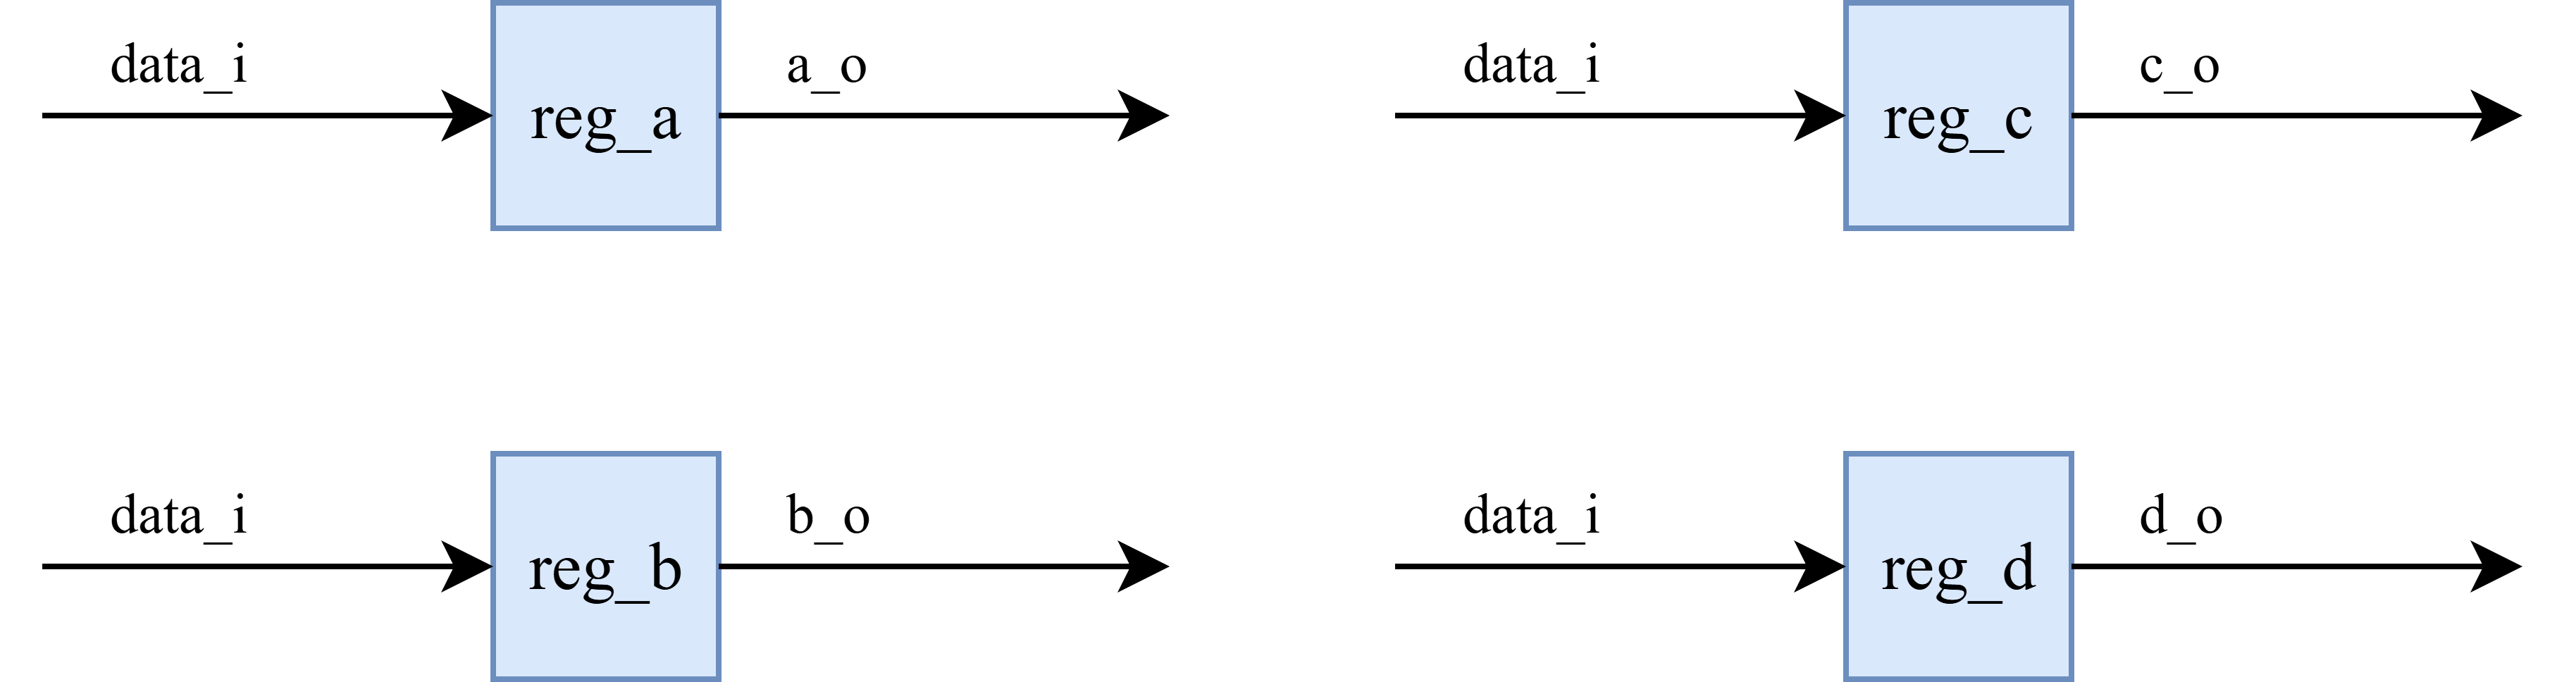
\includegraphics[width=\linewidth]{assets/in_wrap_dp.png}
    \caption{Datapath for input wrapper.}
    \label{fig:q2_in_wrap_dp}
\end{figure}

\begin{table}[h]
    \centering
    \renewcommand{\arraystretch}{1.2}
    \setlength{\tabcolsep}{8pt}

    \begin{tabularx}{\textwidth}{@{}lX@{}}
        \toprule
        \textbf{Signal} & \textbf{Description} \\
        \midrule
        \texttt{en\_a}          & Enable synchronized writing into the \texttt{a} register. \\
        \texttt{en\_b}          & Enable synchronized writing into the \texttt{b} register. \\
        \texttt{en\_c}          & Enable synchronized writing into the \texttt{c} register. \\
        \texttt{en\_d}          & Enable synchronized writing into the \texttt{d} register. \\
        \bottomrule
    \end{tabularx}

    \caption{Control signals for input wrapper datapath.}
    \label{tab:q2_in_wrap_sig}
\end{table}

\begin{figure}[h]
    \centering
    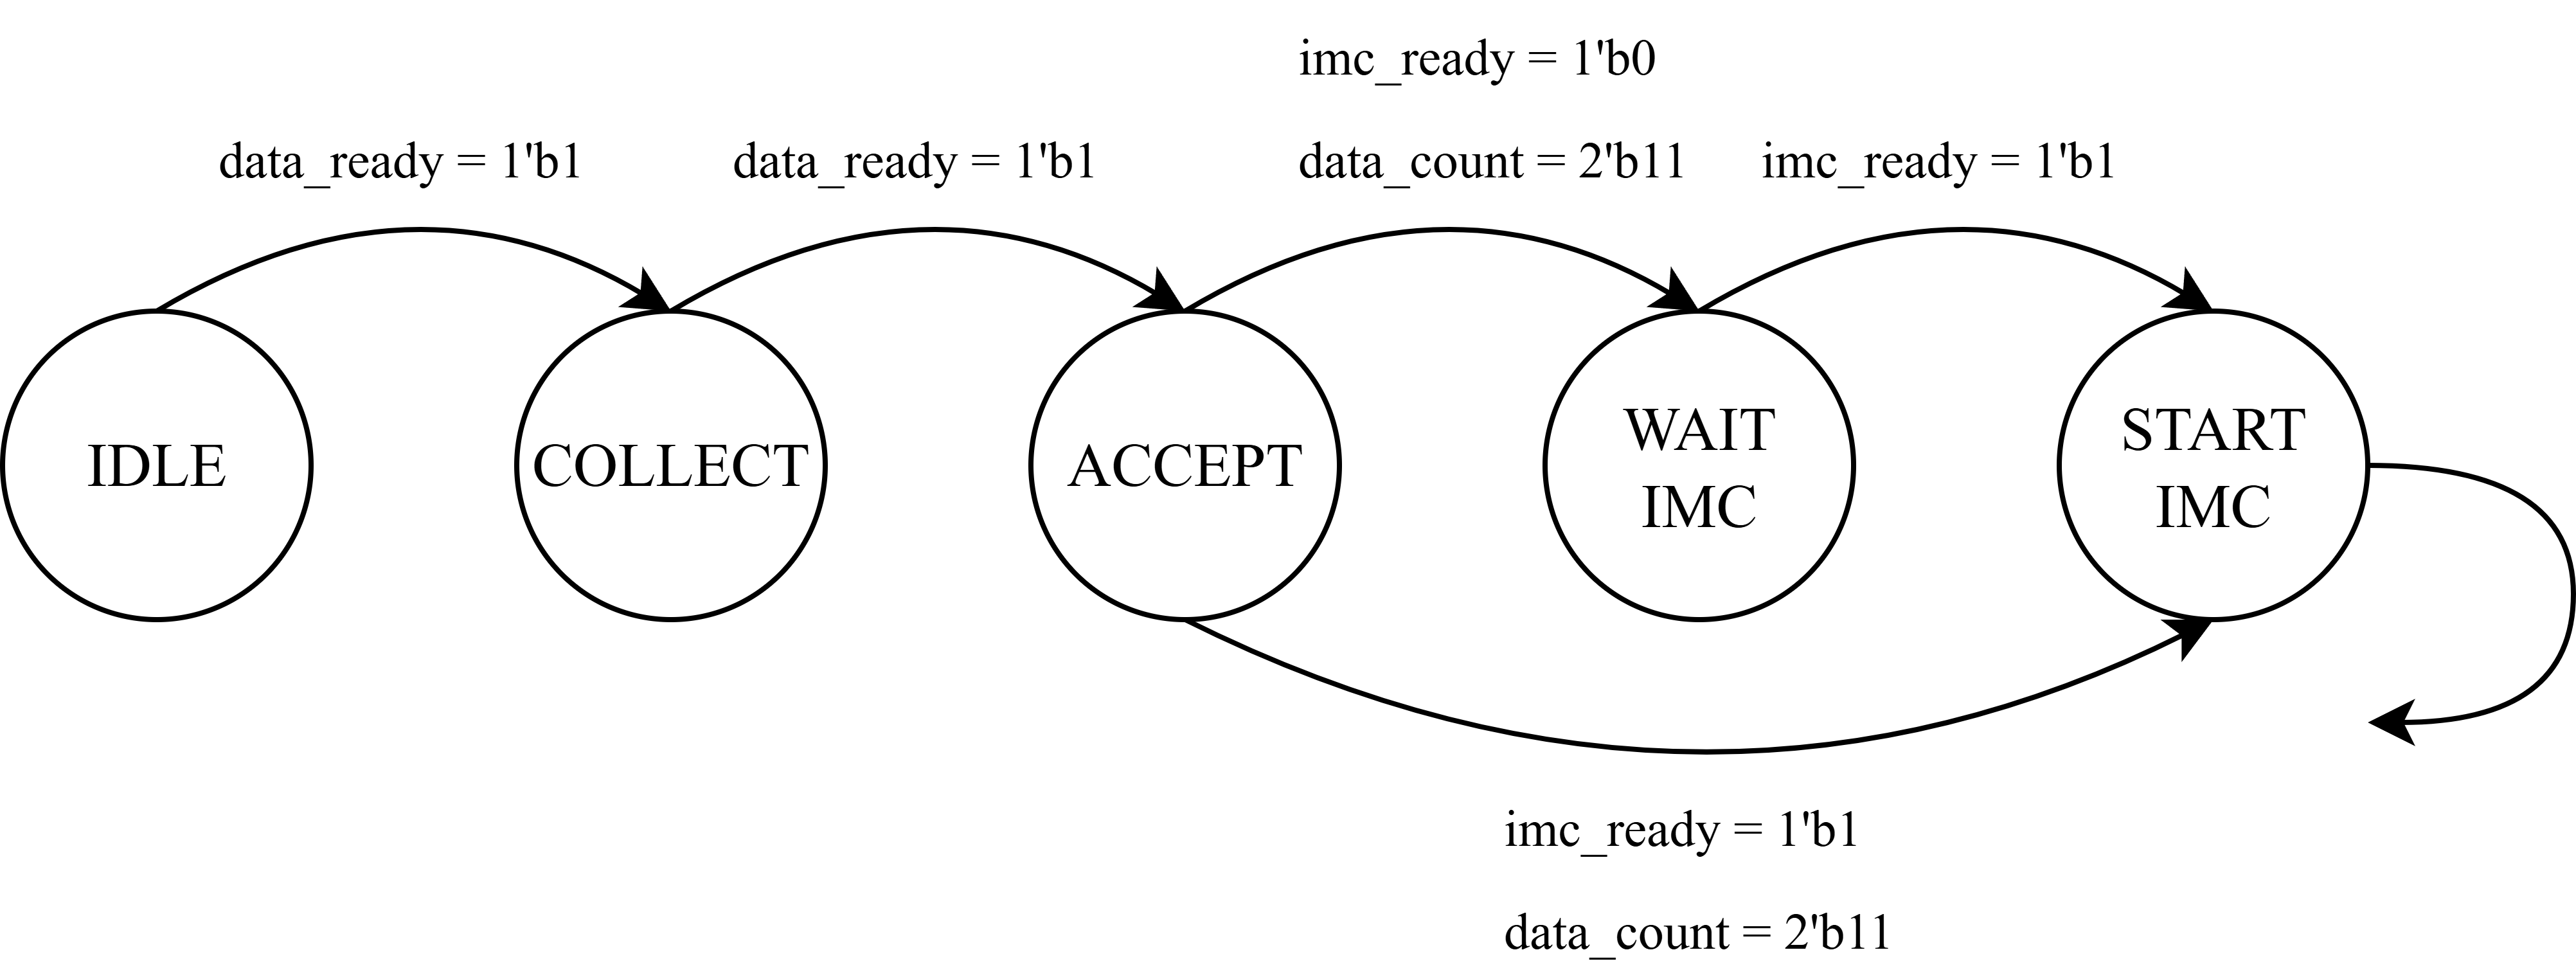
\includegraphics[width=\linewidth]{assets/in_wrap_cont.png}
    \caption{Controller for input wrapper.}
    \label{fig:q2_in_wrap_cont}
\end{figure}

\newpage

The control signal asserted in each state is summarized in \cref{tab:in_wrapper_state_signals} and the testbench waveform is shown in \cref{fig:q2_in_wrapper_wave}.

\begin{table}[h]
    \centering
    \renewcommand{\arraystretch}{1.5}
    \setlength{\tabcolsep}{6pt}

    \begin{tabularx}{\textwidth}{@{}l X@{}}
        \toprule
        \textbf{State} & \textbf{Signals Active (1'b1)} \\
        \midrule
        \texttt{STATE\_IDLE} & 
            None \\ 
        \hline
        \texttt{STATE\_COLLECT} & 
            \texttt{en\_a} (if \texttt{data\_count}=0) \newline
            \texttt{en\_b} (if \texttt{data\_count}=1) \newline
            \texttt{en\_c} (if \texttt{data\_count}=2) \newline
            \texttt{en\_d} (if \texttt{data\_count}=3) \\
        \hline
        \texttt{STATE\_ACCEPT} & 
            \texttt{data\_accept} \\
        \hline
        \texttt{STATE\_WAIT\_IMC} & 
            None \\
        \hline
        \texttt{STATE\_START\_IMC} & 
            \texttt{imc\_start} \\
        \bottomrule
    \end{tabularx}

    \caption{Signals issued in each state of the input wrapper controller.}
    \label{tab:in_wrapper_state_signals}
\end{table}

\begin{figure}[h]
    \centering
    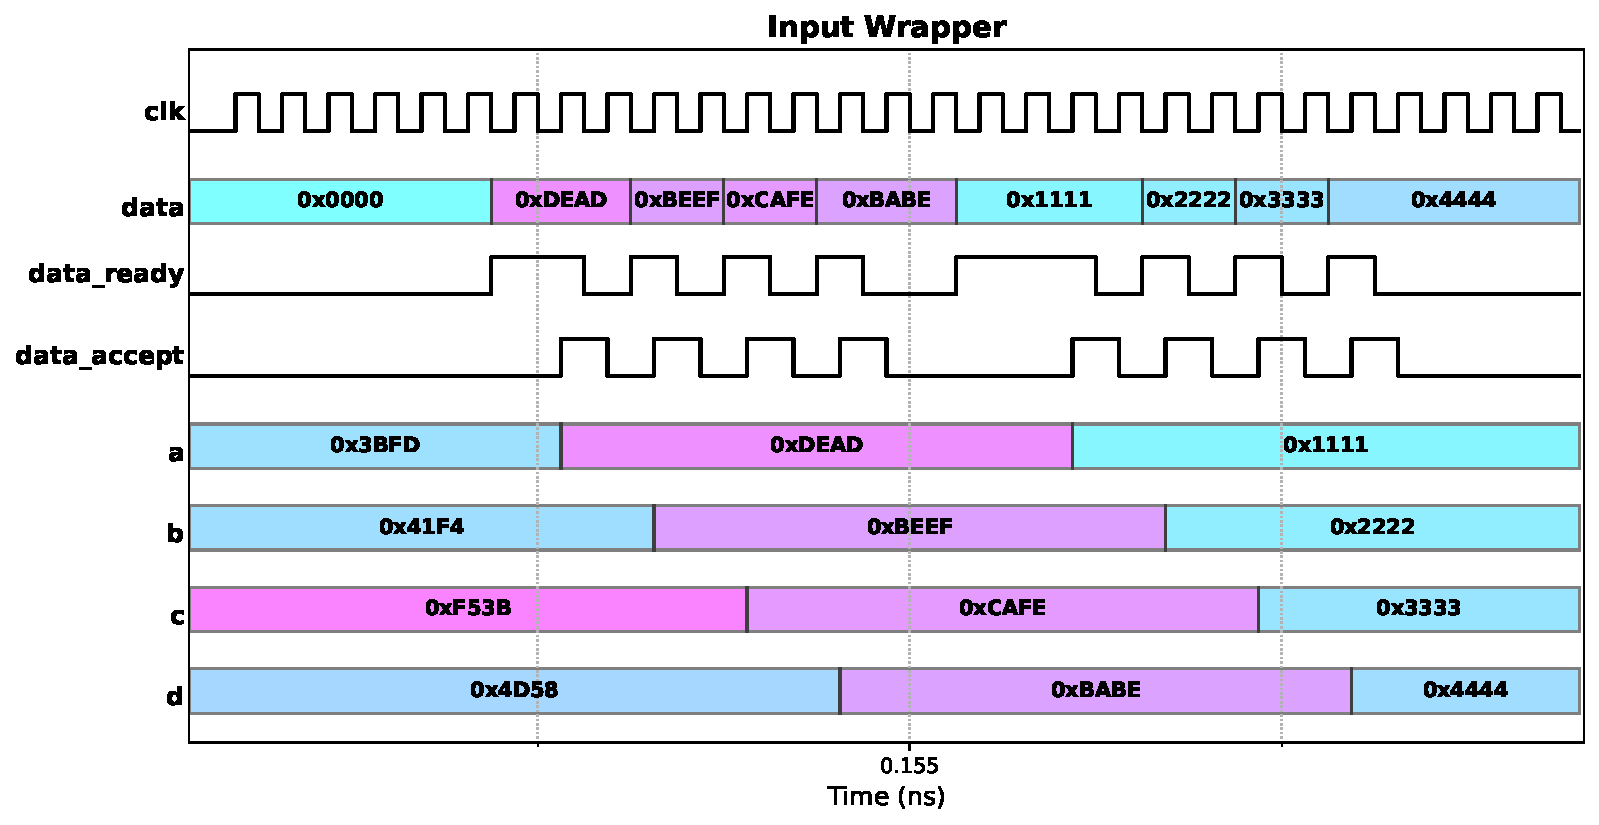
\includegraphics[width=\linewidth]{assets/q2_in_wrapper_wave.pdf}
    \caption{Waveform for input wrapper testbench.}
    \label{fig:q2_in_wrapper_wave}
\end{figure}

\newpage

\subsection*{Output Wrapper}

The output wrapper must be able to store the result from the IMC when it is available and signal an external device that data is available. The datapath consists of four registers to store the results, a 4-to-1 multiplexer to select one for the bus, and a tri-state block to put high-z on the output when it is not driving the bus. The datapath is shown in \cref{fig:q2_out_wrap_dp}. The datapath has three control signals [\cref{tab:q2_out_wrap_sig}]. The controller has four states: \texttt{IDLE}, \texttt{READY}, \texttt{REQUEST\_BUS}, and \texttt{TRANSMIT}. When the IMC asserts \texttt{ready}, the output wrapper latches the outputs to the internal registers and asserts \texttt{available} to external devices. When an external device then requests a transmission by \texttt{start\_transmit}, the wrapper requests access to the bus by asserting \texttt{request} in the \texttt{REQUEST\_BUS} state. When the wrapper is granted access it changes state to \texttt{TRANSMIT}, where an internal counter, \texttt{data\_count}, keeps track of which registers to output. The transition diagram is shown in \cref{fig:q2_out_wrap_cont}. The control signals asserted in each state are summarized in \cref{tab:q2_out_wrap_sig} and the testbench waveform is shown in \cref{fig:q2_out_wrapper_wave}.

\begin{figure}[h]
    \centering
    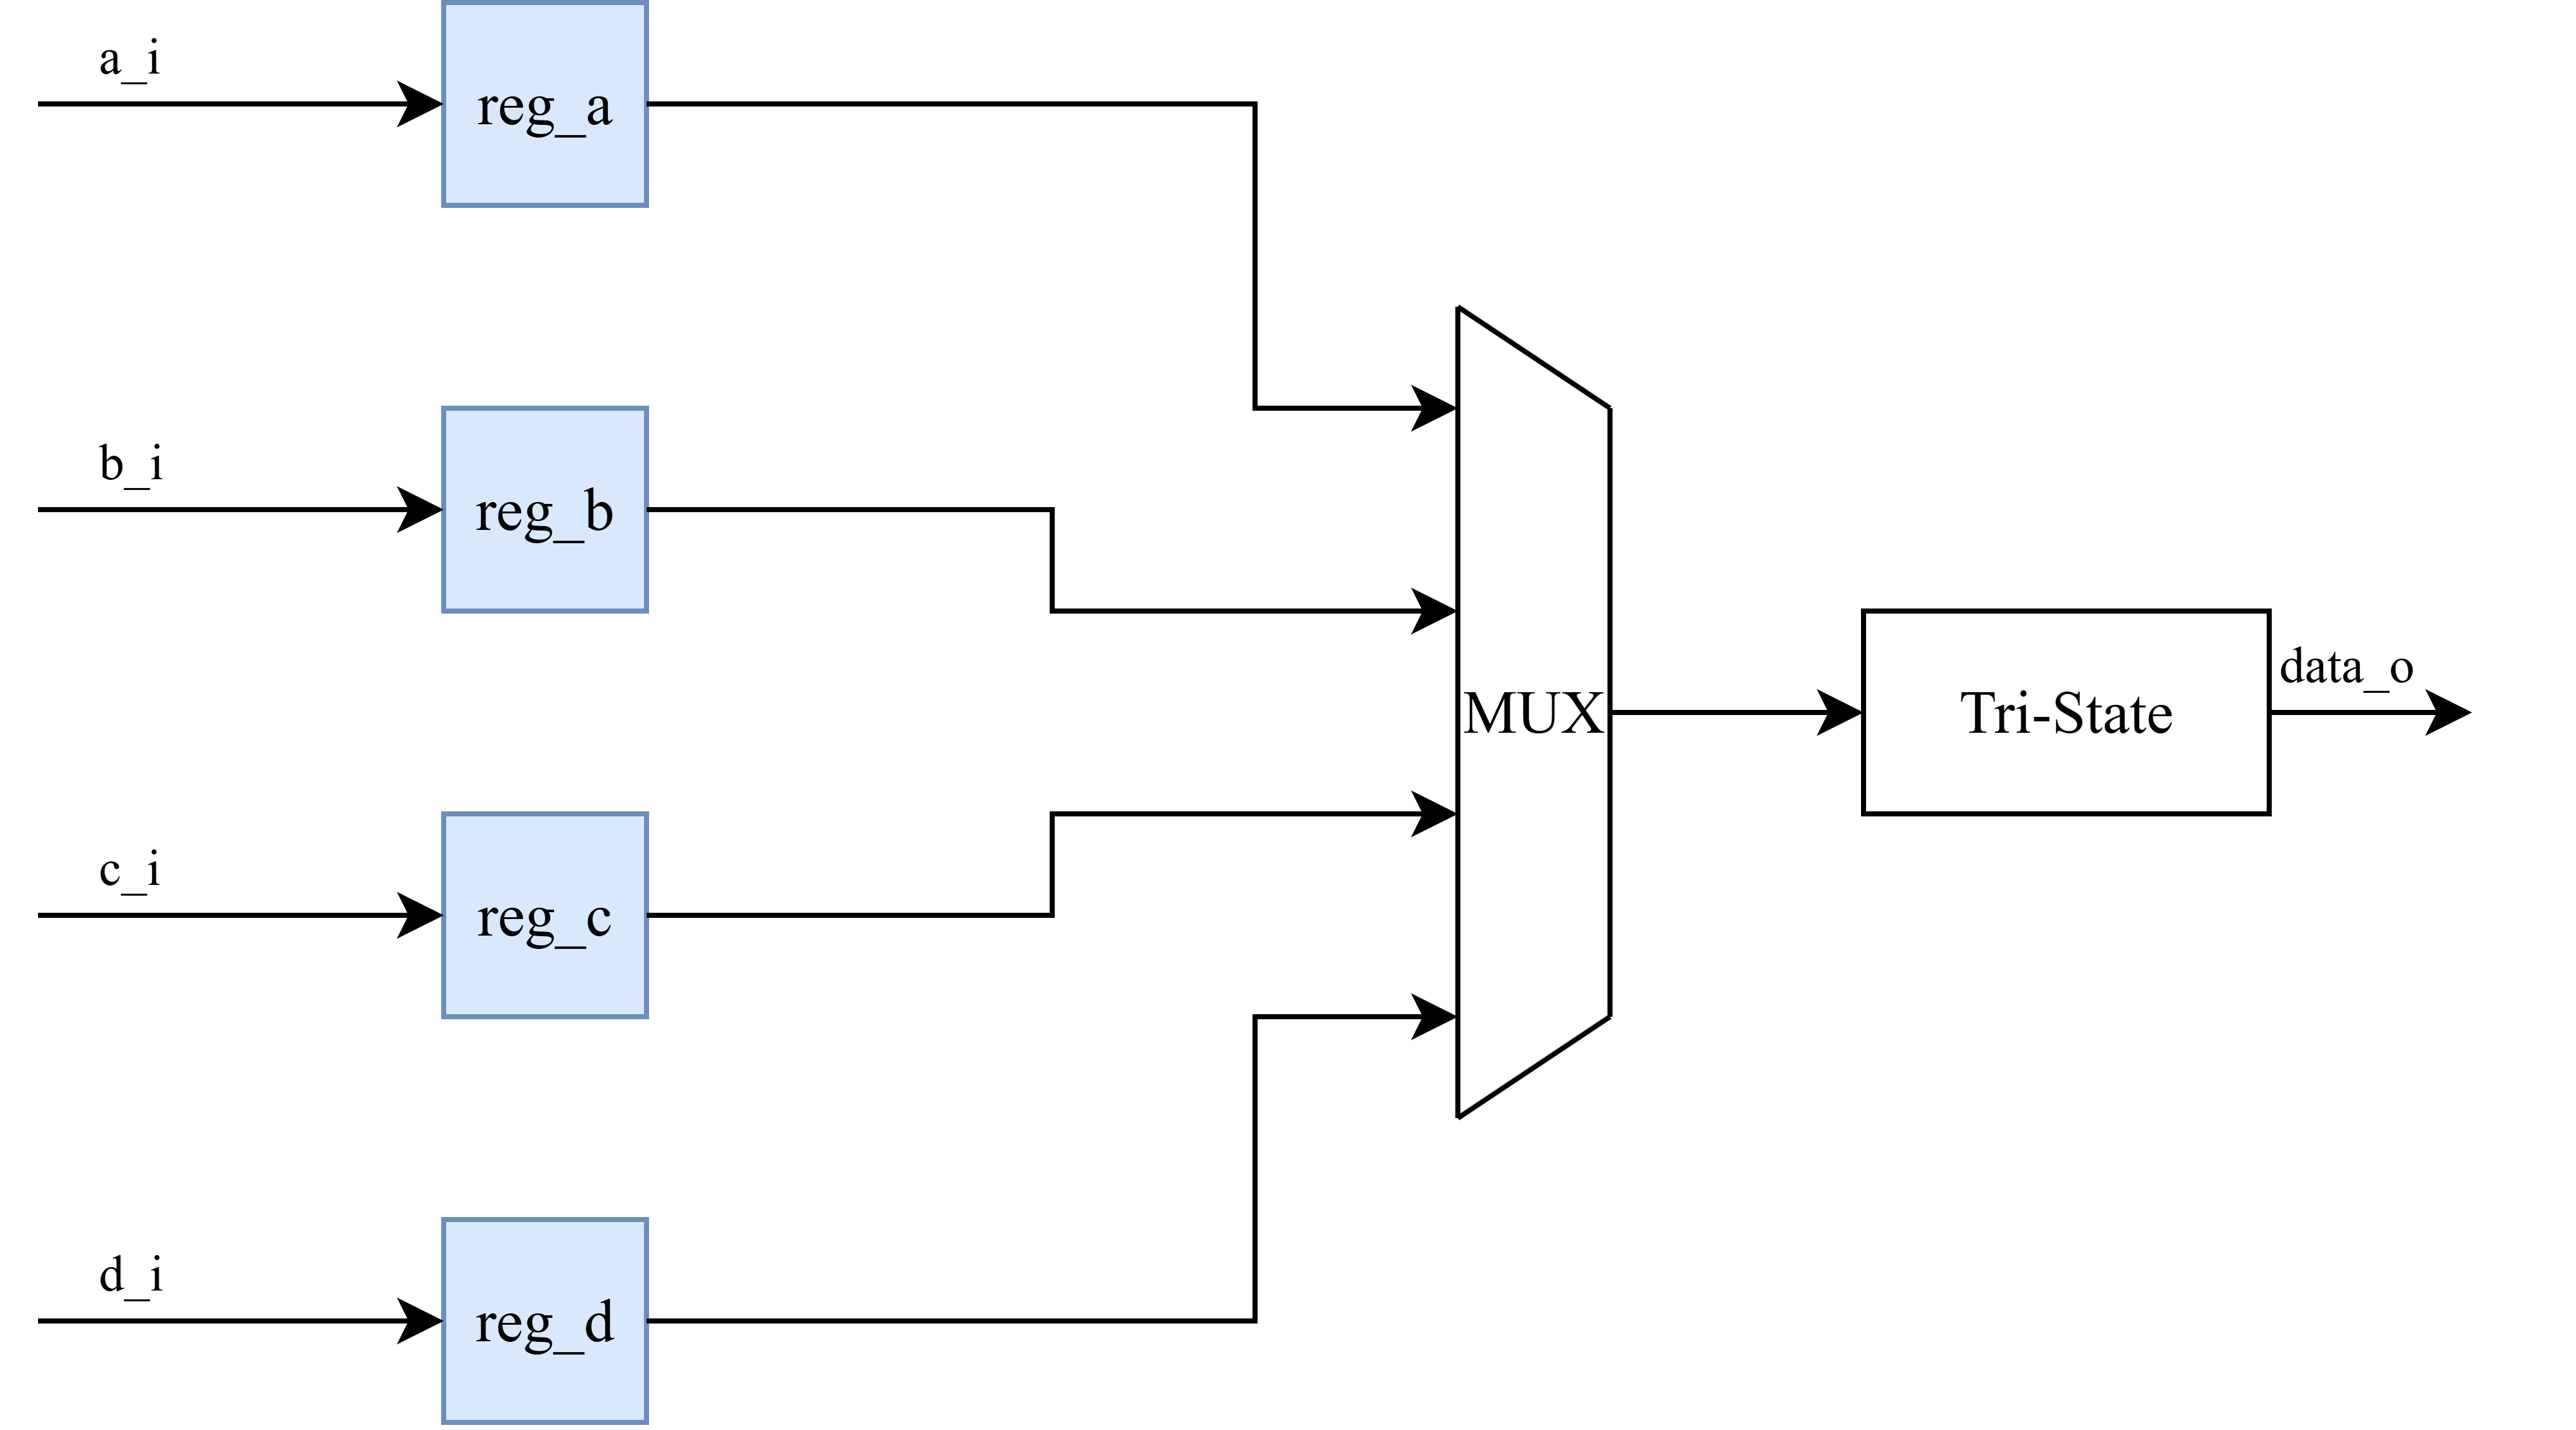
\includegraphics[width=\linewidth]{assets/out_wrap_dp.png}
    \caption{Datapath for output wrapper.}
    \label{fig:q2_out_wrap_dp}
\end{figure}

\begin{table}[h]
    \centering
    \renewcommand{\arraystretch}{1.2}
    \setlength{\tabcolsep}{8pt}

    \begin{tabularx}{\textwidth}{@{}lX@{}}
        \toprule
        \textbf{Signal} & \textbf{Description} \\
        \midrule
        \texttt{drive\_bus} & 1'b0: High-z, \hspace{20pt} 1'b1: Passes the MUX output to the bus \\
        \texttt{latch\_imc} & Enable synchronized writing into the \texttt{a}, \texttt{b}, \texttt{c}, and \texttt{d} registers. \\
        \texttt{data\_mux}  & Outputs the corresponding register to the tri-state block. \\
        \bottomrule
    \end{tabularx}

    \caption{Control signals for input wrapper datapath.}
    \label{tab:q2_out_wrap_sig}
\end{table}

\newpage

\begin{figure}[h]
    \centering
    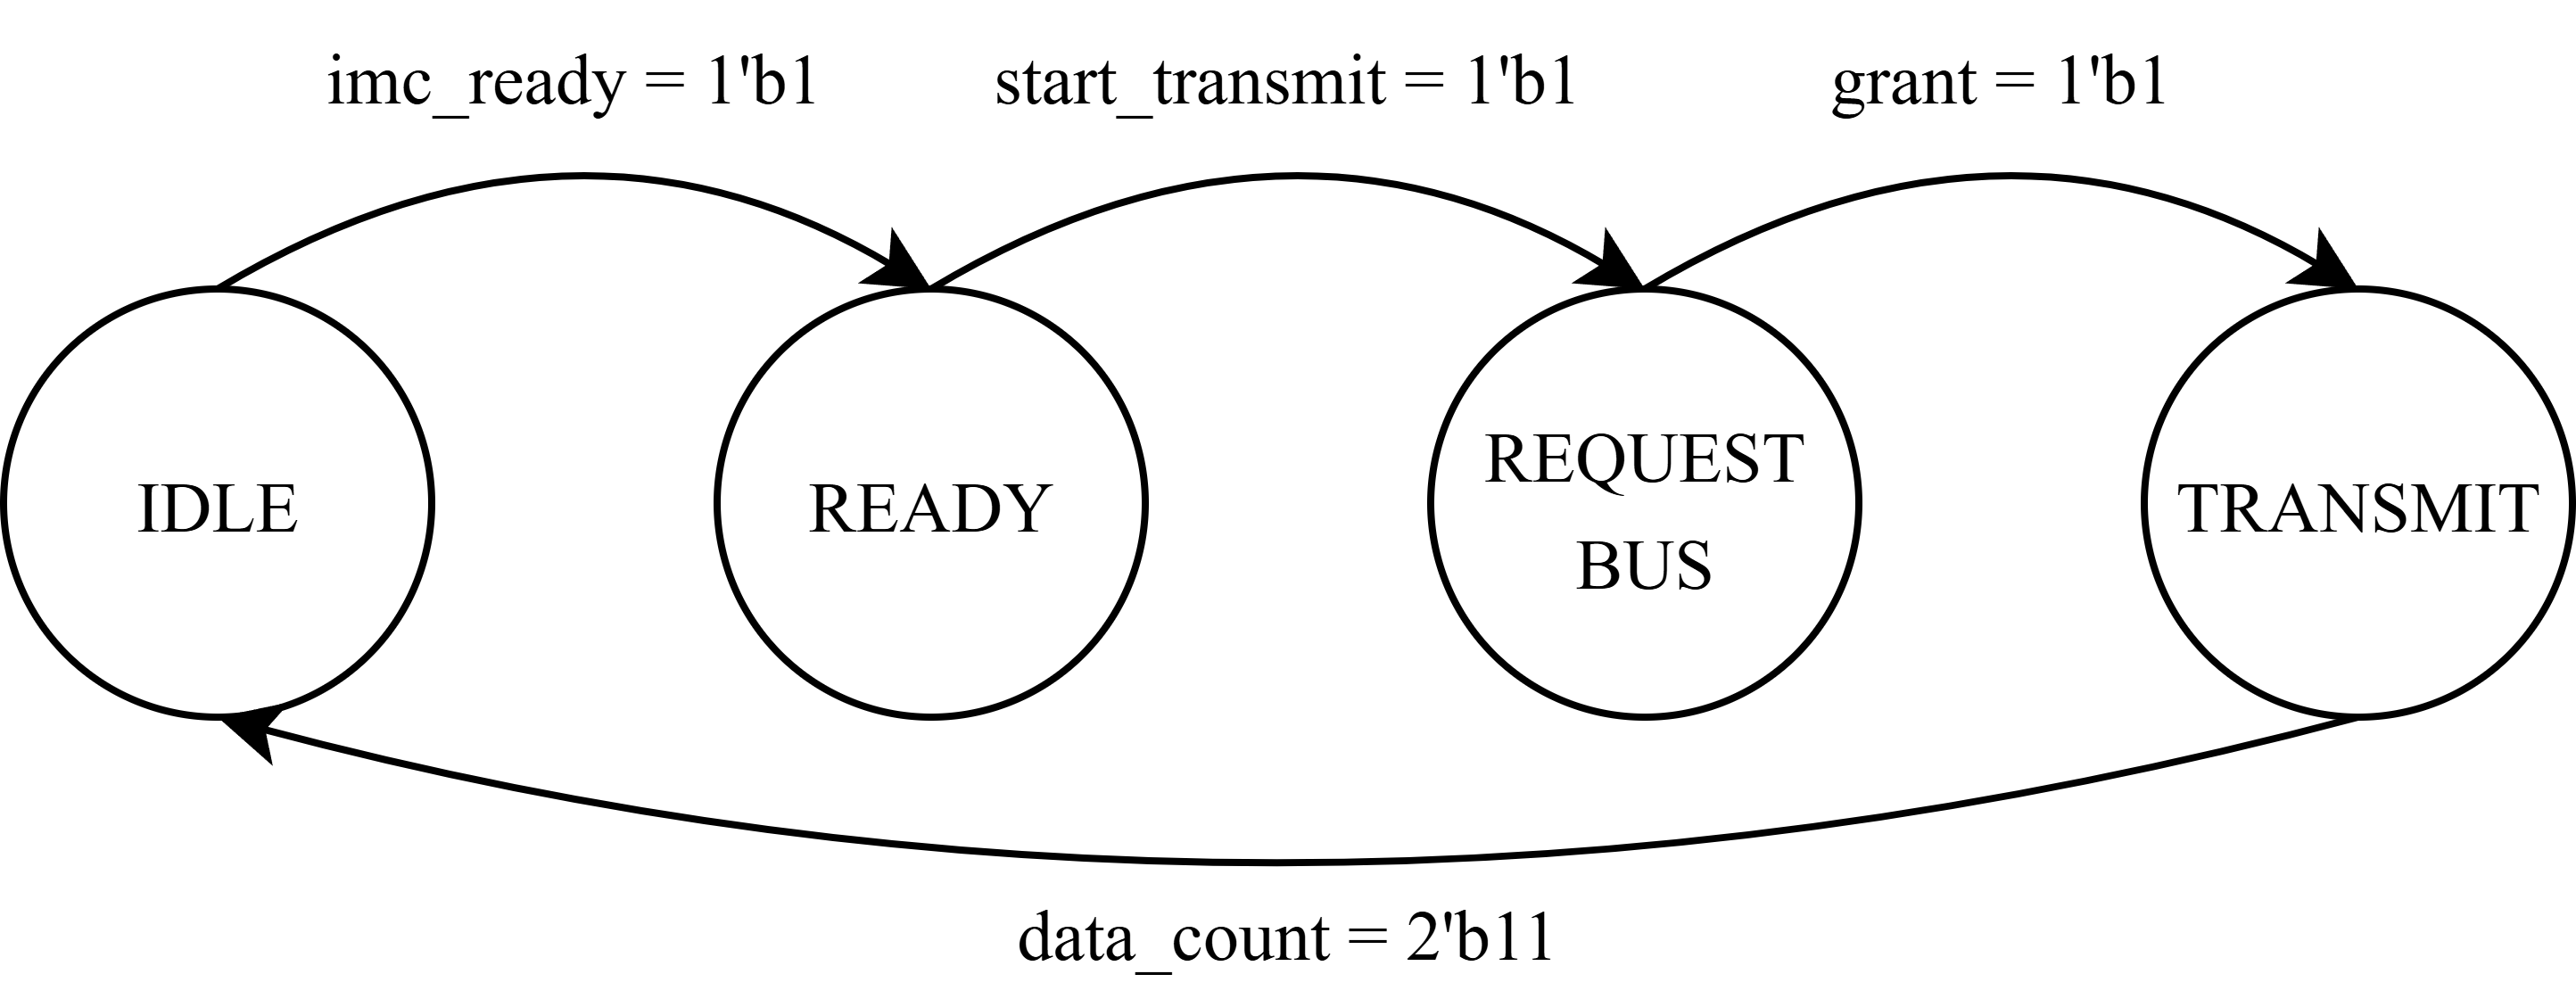
\includegraphics[width=0.8\linewidth]{assets/out_wrap_cont.png}
    \caption{Datapath for output wrapper.}
    \label{fig:q2_out_wrap_cont}
\end{figure}

\begin{table}[h]
    \centering
    \renewcommand{\arraystretch}{1.5}
    \setlength{\tabcolsep}{6pt}

    \begin{tabularx}{\textwidth}{@{}l X@{}}
        \toprule
        \textbf{State} & \textbf{Signals Active (1'b1)} \\
        \midrule
        \texttt{STATE\_IDLE} & 
            None \\ 
        \hline
        \texttt{STATE\_READY} & 
            \texttt{avail} \newline
            \texttt{latch\_imc} \\
        \hline
        \texttt{STATE\_REQUEST\_BUS} & 
            \texttt{request} \\
        \hline
        \texttt{STATE\_TRANSMIT} & 
            \texttt{ready} \newline
            \texttt{drive\_bus} \newline
            \texttt{data\_mux} (selects \texttt{a}, \texttt{b}, \texttt{c}, \texttt{d} based on \texttt{data\_count}) \\
        \bottomrule
    \end{tabularx}

    \caption{Signals issued in each state of the output wrapper controller.}
    \label{tab:out_wrapper_state_signals}
\end{table}

\begin{figure}[H]
    \centering
    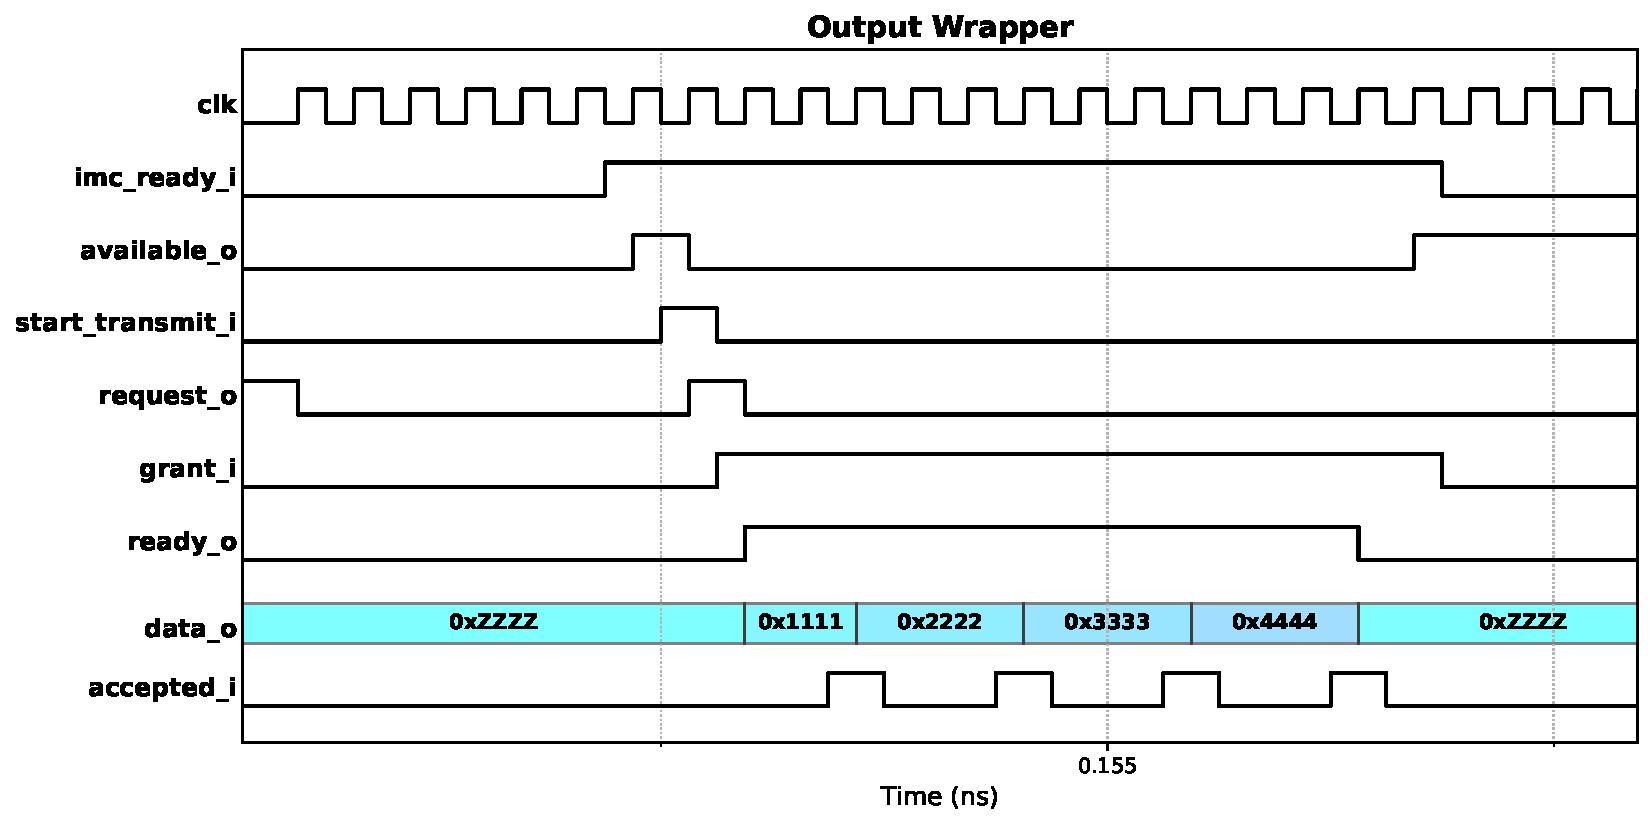
\includegraphics[width=\linewidth]{assets/q2_out_wrapper_wave.pdf}
    \caption{Waveform for output wrapper testbench.}
    \label{fig:q2_out_wrapper_wave}
\end{figure}

\newpage

\section{Question 3}

You are to design an interface circuit for device $A$ with a 64-bit data bus (dataA) that is to write to device $B$, which receives 8-bit data through and arbitrated 8-bit shared bus (sharedBus). The interface circuit is called IAB and communicates with device $A$ by fully responsive two-line handshaking initiated by device A (readyA, when A is to write, and acceptedA when the 64-bit data is received by IAB). The interface circuit requests the use of the sharedBus by issuing reqIAB and waits for gntIAB before it can use the bus. When IAB has access to the bus, it writes the 64-bit data it received from $A$ in eigth 8-bit chunks to device $B$ in a burst. For each write to $B$, IAB communicates with device $B$ by fully responsive twoline handshaking initiated by IAB (readyI, when IAB is to wrtie, and acceptedI when the 8-bit is received by device $B$).

\begin{enumerate}
    \item Draw the block diagram of the completed system, including your circuits' input and output bus, shared bus, and the bus between thetwo devices and your interface circuit.
    \item Draw the complete datapath of IAB, including the components and necessary internal control signals.
    \item Draw a state diagram showing the IAB controller's behavior. In each state show the control signals that are issued.
    \item Draw wiring between the datapath and controller.
    \item Model the datapath, controller, and the IAB interface in SystemVerilog.
    \item Verify the design with a testbench.
\end{enumerate}

\subsection*{Solution}

The block diagram of the system is shown in \cref{fig:q3}. The datapath consists of a single 64-bit register for storing the value from $A$, and a multiplexer and tri-state block for outputting the corresponding 8-bits to the shared 8-bit bus. The datapath and it's control signals are shown in \cref{fig:q3_dp} and \cref{tab:q3_sig}.

\begin{figure}[H]
    \centering
    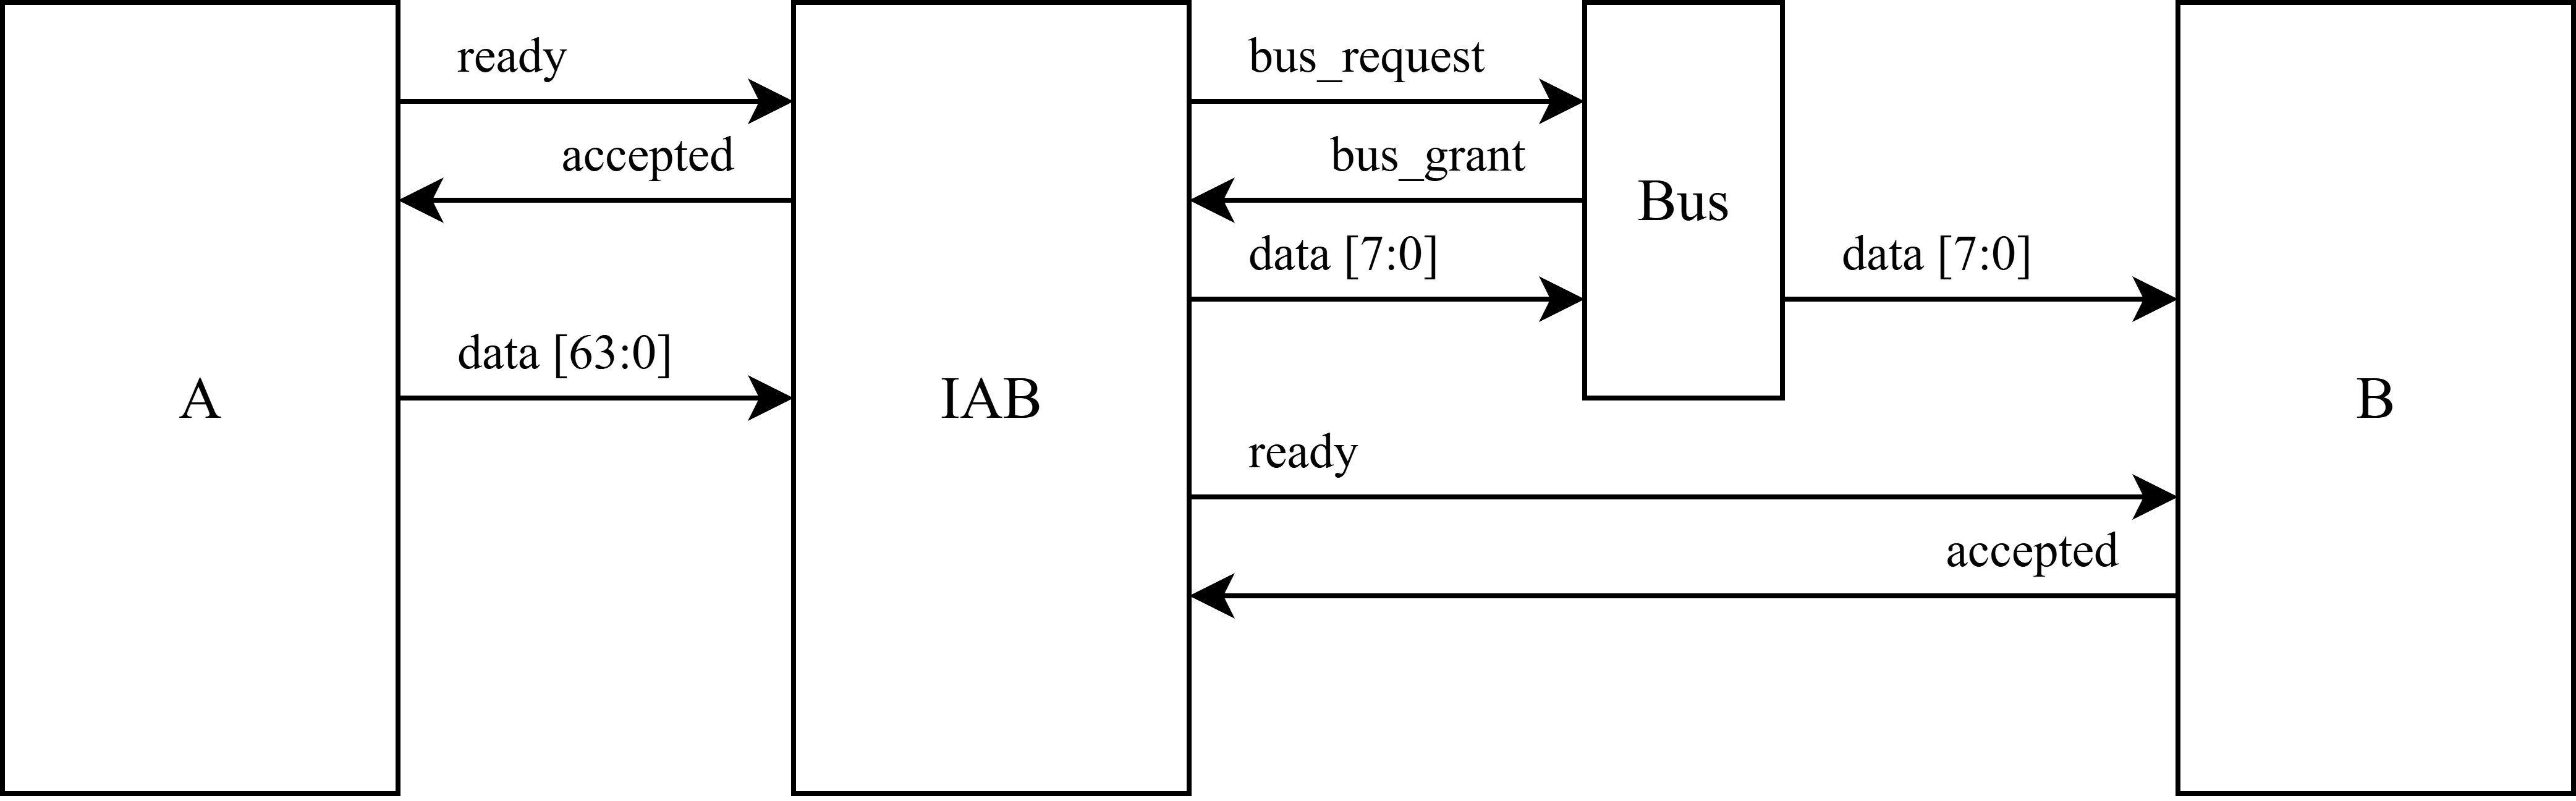
\includegraphics[width=\linewidth]{assets/q3.png}
    \caption{Block diagram of IAB.}
    \label{fig:q3}
\end{figure}

\newpage

\begin{figure}[h]
    \centering
    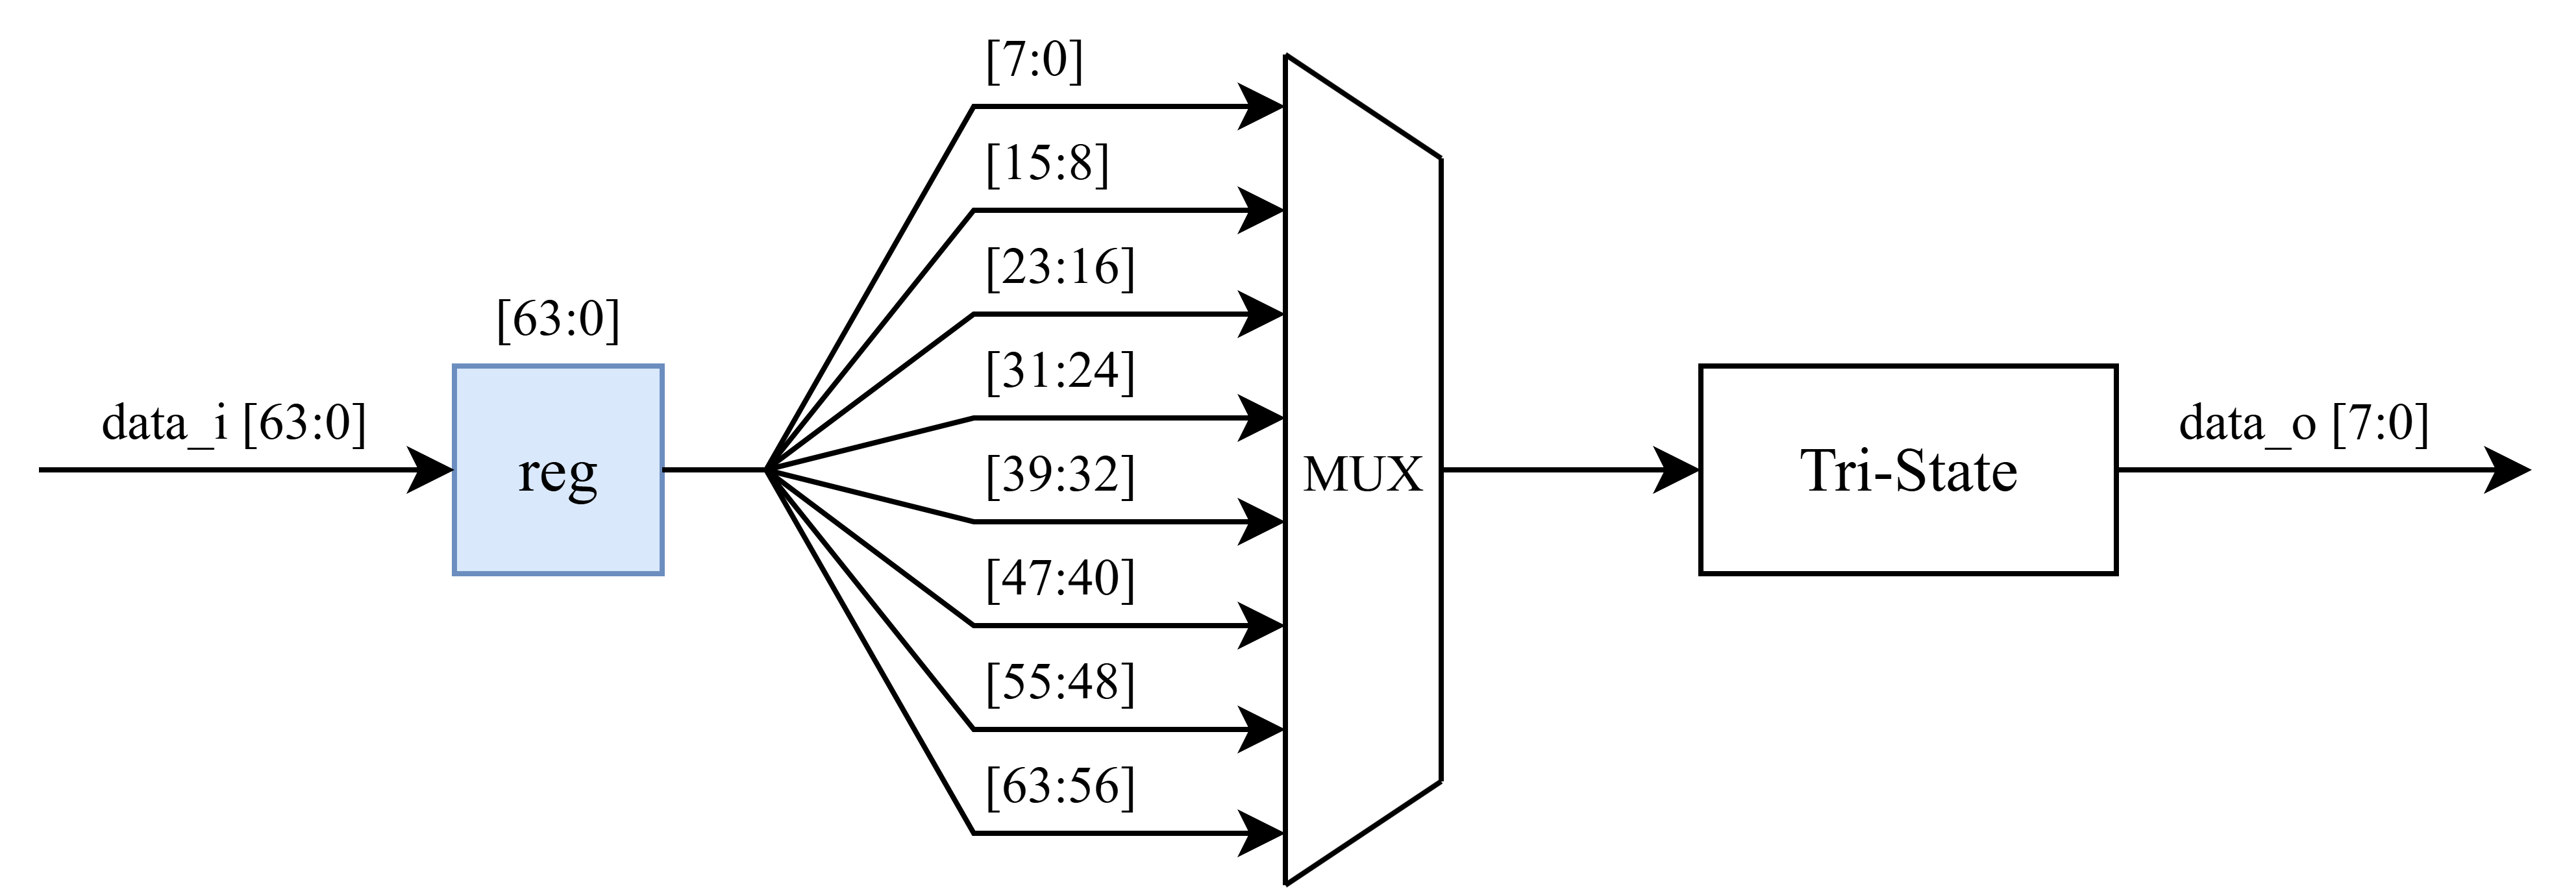
\includegraphics[width=\linewidth]{assets/q3_dp.png}
    \caption{Datapath of IAB.}
    \label{fig:q3_dp}
\end{figure}

\begin{table}[h]
    \centering
    \renewcommand{\arraystretch}{1.2}
    \setlength{\tabcolsep}{8pt}

    \begin{tabularx}{\textwidth}{@{}lX@{}}
        \toprule
        \textbf{Signal} & \textbf{Description} \\
        \midrule
        \texttt{latch}      & Stores the data from A in the register.           \\
        \texttt{mux [2:0]}  & Outputs the corresponding 8-bits of the register. \\
        \texttt{drive\_bus} & Enables data to pass through the tri-state block. \\
        \bottomrule
    \end{tabularx}

    \caption{Control signals for IAB datapath.}
    \label{tab:q3_sig}
\end{table}

\begin{figure}[h]
    \centering
    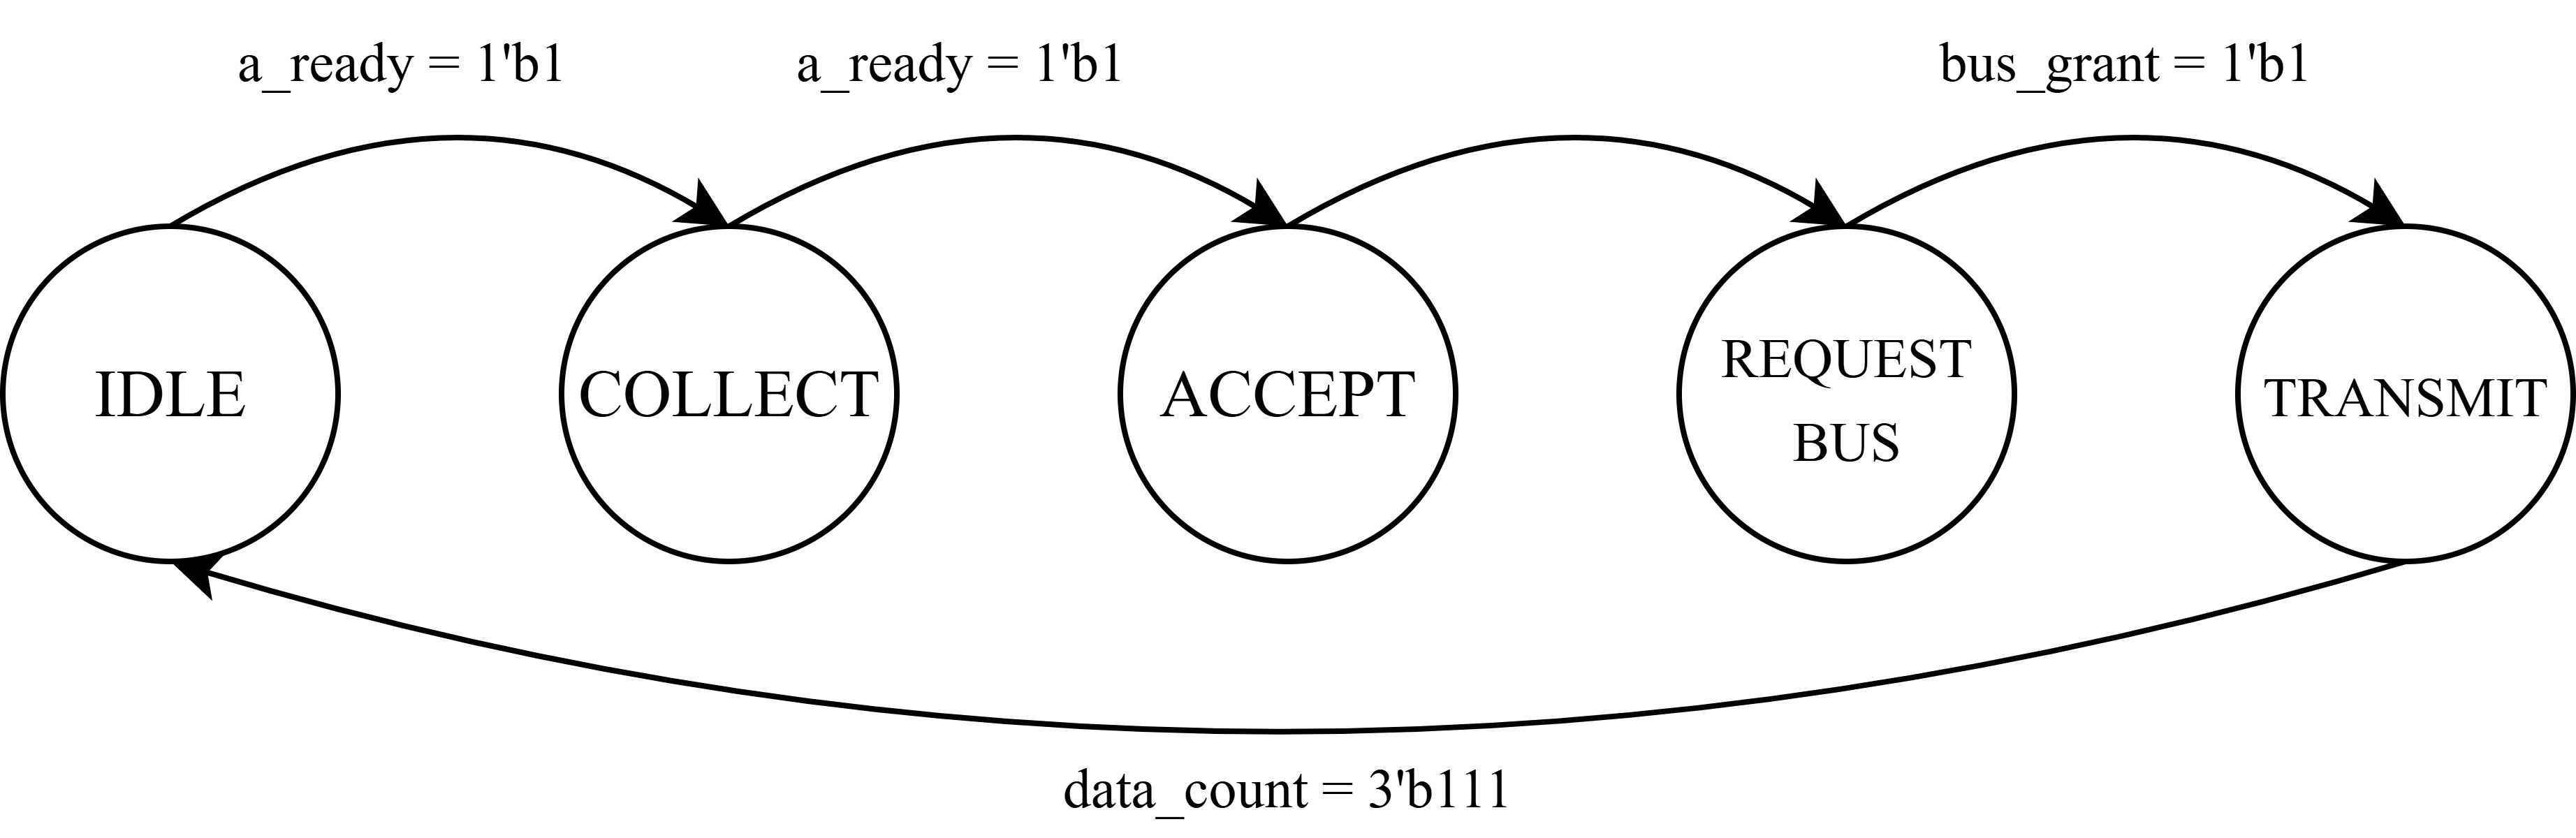
\includegraphics[width=\linewidth]{assets/q3_cont.png}
    \caption{IAB controller state transitions.}
    \label{fig:q3_cont}
\end{figure}

The controller consists of 5 states: \texttt{IDLE}, \texttt{COLLECT}, \texttt{ACCEPT}, \texttt{REQUEST\_BUS}, and \texttt{TRANSMIT}. When $A$ signals it has data ready, the controller moves to the \texttt{COLLECT} state where the value is then stored in the datapath register. Afterwards it moves to \texttt{ACCEPT} and outputs the handshake accept signal. After accepting data from $A$, it moves to \texttt{REQUEST\_BUS} where it asserts a \texttt{bus\_req} signal and waits \texttt{bus\_grant}. When bus access has been granted, the controller switches to its last state, \texttt{TRANSMIT}, where it starts driving the shared bus. An internal counter, \texttt{data\_count}, keeps track of which 8-bit value from the 64-bit data register to output. The signals asserted in each state are summarized in \cref{tab:iab_controller_state_signals}. To verify the IAB module, a testbench was created that simulates the expected stimuli. A value of 0x1122334455667788 is sent from $A$. The testbench output and waveform is shown on the next page.

\newpage

\vspace{-10pt}
\begin{table}[h]
    \centering
    \renewcommand{\arraystretch}{1.5}
    \setlength{\tabcolsep}{6pt}

    \begin{tabularx}{\textwidth}{@{}l X@{}}
        \toprule
        \textbf{State} & \textbf{Signals Active (1'b1)} \\
        \midrule
        \texttt{STATE\_IDLE} & 
            None \\
        \hline
        \texttt{STATE\_COLLECT} & 
            \texttt{latch} \\
        \hline
        \texttt{STATE\_ACCEPT} & 
            \texttt{accepted\_a} \\
        \hline
        \texttt{STATE\_REQUEST\_BUS} & 
            \texttt{bus\_req} \\
        \hline
        \texttt{STATE\_TRANSMIT} & 
            \texttt{ready} \newline
            \texttt{drive\_bus} \newline
            \texttt{mux} (counts from 0 to 7 based on \texttt{data\_count}) \\
        \bottomrule
    \end{tabularx}

    \caption{Signals issued in each state of the IAB controller.}
    \label{tab:iab_controller_state_signals}
\end{table}

\vspace{-10pt}
\begin{textcode}{q3 - IAB testbench output}
[60] Reset...
[80] IAB accepted 64-bit data from A
[90] IAB requested bus
[100] Bus granted to IAB
[110] IAB sent 0: 0x88
[140] IAB sent 1: 0x77
[170] IAB sent 2: 0x66
[200] IAB sent 3: 0x55
[230] IAB sent 4: 0x44
[260] IAB sent 5: 0x33
[290] IAB sent 6: 0x22
[320] IAB sent 7: 0x11
[350] Completed transfer
\end{textcode}

\vspace{-10pt}
\begin{figure}[H]
    \centering
    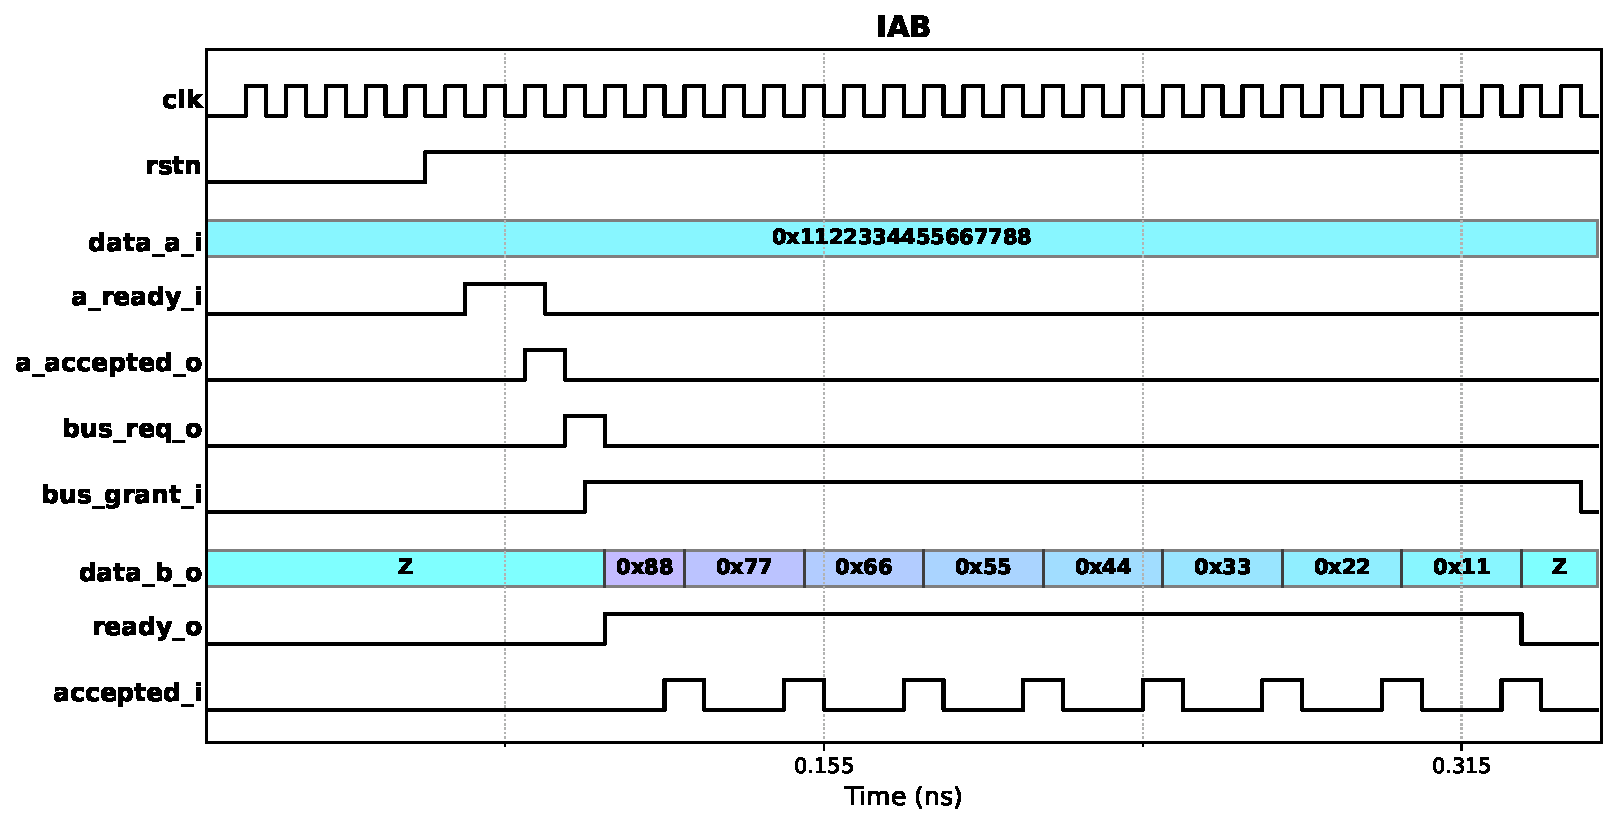
\includegraphics[width=\linewidth]{assets/q3_wave.pdf}
    \caption{Waveform for IAB testbench.}
    \label{fig:q3_wave}
\end{figure}

\newpage

\section{Question 4}

You are to generate constrained random test data for the CPU-memory interface shown below, which you have previously seen in Milestones 3 and 4. In this exercise, the CPU performs burst transfers when reading from or writing to memory.

A burst access is a sequence of consecutive trasnfers. In this scenario, we do bursts without an explicit \texttt{burst} signal. We just handle bursts internally by generating one transaction with $\text{burst\_len} = N$, driving \texttt{read\_en} or \texttt{write\_en} high for $N$ consecutive cycles, and incrementing the address by 4 each cycle.

Define the following constraints to control randomization behavior.

\begin{itemize}
    \item \textbf{Burst Length Constraint}: Limits the number of data items in a burst to between 2 and 8 transfers.
    \item \textbf{Address Alignment Constraint}: Ensures the address is word-aligned (4-byte aligned).
    \item \textbf{Address Range Partitioning}: Assigns different memory regions for read and write operations. Memory region for reading is \texttt{[32'h0000\_0000:32'h0000\_FFFF]}. The region for writing is \texttt{[32'h1000\_0000:32'h1000\_FFFF]}.
    \item \textbf{Operation Probability}: Randomly selects read or write operations with weighted probability:
    \begin{itemize}
        \item 80\% chance to generate a read
        \item 20\% chance to generate a write
    \end{itemize}
    \item \textbf{Write Enable Constraint}: Ensured valid \texttt{write\_en} values only for write transfers. At least one byte must be enabled (non-zero pattern). For read transfers, \texttt{write\_en} must be zero. The 4 bits of write enable are used for the four bytes in the addressed word. Only the 8 values 0000, 1111, 1100, 0011, 1000, 0100, 0010, and 0001 are possible, i.e. no write, write 32 bits, write upper 16 bits, write lower 16, or write a single byte, respectively.
\end{itemize}

\subsection*{Solution}



\end{document}
